\documentclass[a4paper]{report}
\usepackage{graphicx}
\usepackage{array}
\usepackage{natbib}
\usepackage{hyperref}
\usepackage[english]{babel}
\usepackage{lscape}

\begin{document}
\begin{titlepage}
\begin{center}
\textsc{\LARGE Contextproject Programming Life}\\
\vspace{5pt}
\textsc{\LARGE Group 2 - GEVATT}\\
\vspace{5pt}
\textsc{\LARGE Final Report}\\
\vspace{5pt}
\textsc{\large TU Delft}

\begin{table}[ht]
\centering
\begin{tabular}{ccc}

\includegraphics[scale=0.2]{ruben.png}   &
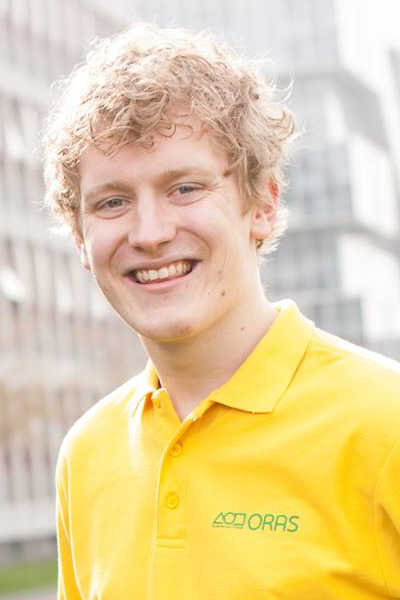
\includegraphics[scale=0.2]{mathijs.png} &

\includegraphics[scale=0.2]{jasper.png}  \\
Ruben Bes	& Mathijs Hoogland	& Jasper Denkers\\
rbes 		& mhhoogland 		& jdenkers\\
4227492 	& 4237676 			& 4212584\\
\end{tabular}
\end{table}

\begin{table}[ht]
\centering
\begin{tabular}{cc}
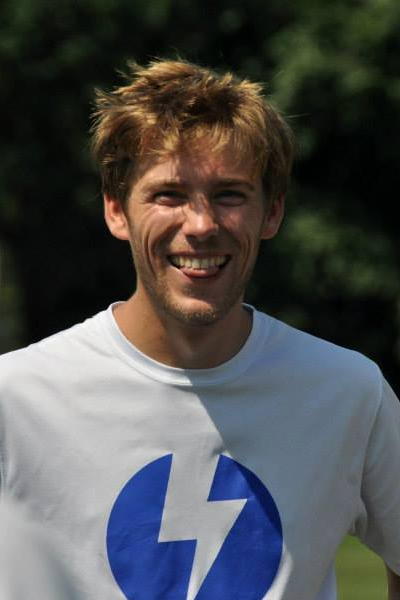
\includegraphics[scale=0.2]{robbert.png} &

\includegraphics[scale=0.2]{willem.png}  \\
Robbert van Staveren	& Willem Jan Glerum\\
rhvanstaveren 			& wglerum\\
1527118					& 4141040\\
\end{tabular}
\end{table}

\vfill
{\large \today}
\end{center}

\end{titlepage}

\begin{landscape}
\setlength\extrarowheight{5pt}
\begin{table}[ht]
\begin{tabular}{p{6cm}|l|l|l|p{2cm}|p{7cm}}

\textbf{Task} & \textbf{Effort} & \textbf{Assignment} & \textbf{Actual effort} & \textbf{Done} & \textbf{Notes}\\
\hline \hline

Work up sprint plan week 5 & 1 & Willem Jan & 1 hour & Yes & None\\
Lookup viualization libraries & 2 & Willem Jan & - & No & No time for it yet\\
Visualize proccessed VCF data overview & 4 & Willem Jan & 8 hours & Yes & Basic overview of mutations per patient\\
Design and setup database for patients records & 4 & Willem Jan & 8 hours & Yes & Made database design, but had some problems with connection. Setup java classes in combination with database and wrote queries to fetch data for these objects. Problems with testing icm with play framework\\
Sprint reflection week 4 & 1 & Ruben & 1 hour & Yes & None\\
Integrate DB connection in PLAY framework & 4 & Ruben & 6 hours & Yes & Had some issues with the pom file\\
Query proteins associated to other proteins & 1 & Ruben & 1 hour & Yes & None\\
Link string and snp database & 3 & Ruben & 6 hours & No & Had issues linking the databases, because of incorrect database schematics. I have received some extra information which will be put to use next week\\
Make login page & 3 & Jasper & 8 hours & Yes & Used Plays built in Security/Authentication framework. Took some time to figer out but worked in the end. Login page built using Bootstrap. Secured pages are redirected to login page when users isn't logged in\\
Make add patient page & 2 & Jasper & 4 hours & Yes & Upload functionality for vcd file might be added. Used same form technique as logging in and therefore was done a bit quicker.\\
Make select patient page & 2 & Jasper & 3 hours & Yes & Used Bootstrap to make a nice overview. Most time was in securing the pages so one user can't acces other users's patients. Also mutation pages added and same story for security here. \\
Implement JSON protocol between server and client & 3 & Jasper & 3 hours & Yes/No & Have implemented a Ajax setup for removing patients. No JSON but when JSON is needed there's little adjustment to make.\\
Implement HTTPS protocol & 3 & Mathijs & & & \\
Setup webapp on a server for demonstration & 1 & Mathijs & & & \\
Integrate VCF proccessing in play & 2 & Robbert & & & \\
Match mutations with proteins & 8 & Robbert & & & \\
\end{tabular}
\end{table}
\end{landscape}
\end{document}